\section{Auswertung}
\label{sec:Auswertung}

Um den Vielkanalanalysator zu kalibrieren werden mit Hilfe eines Doppelimpuls-Generators Impulse
mit unterschiedlichem zeitlichem Abstand eingelesen. Die belegten Kanäle sind in dargestellt
und in gegen die Impulsabstände aufgetragen.
Da das Plateau nicht sehr stark ausgeprägt ist, wurde eine Gaußfunktion höherer Potenz, anstatt einer Rechteckfunktion als Anpassungsfunktion gewählt.
Dementsprechend ist die Halbwertsbreite der angepassten Funktion mit $T_{\text{FWHM}} = \SI{16,4}{\nano \second}$ größer als das eigentliche Plateau.
Die Auflösungszeit~$\symup{\Delta}t_K$ der Koinzidenzapparatur ist gleichbedeutend
mit der Differenz zwischen der Summe der Diskriminatorbreiten und der in grün
eingezeichneten Halbwertsbreite. Zur Bestimmung von dieser wird
ein linearer Fit für das Plateau und die beiden Flanken durchgeführt. Durch die halbe
Höhe des Plateau ist anschließend die Halbwertsbreite gegeben. 



\subsection{Justage}
\label{subsec:Justage}
Es kann in den PMTs, den Kabeln und den  Diskriminatoren bei einem Myonensignal unterschiedliche Verzögerungen enststehen, was dazu führen kann, dass die Koinzidenz kein Signal weitergibt.
Zur Vermeidung gibt es vor den Diskriminatoren die Verzögerungen, die justiert werden. Um die Verzögerung richtig zu justieren wird diese variiert und in einem $\qty{40}{\second}$ Intervall
das Myonensstartsignal gemessen. In \autoref{fig:Verzoegerung} ist das Myonensstartsignal gegenüber der Verzögerung aufgetragen.
\begin{figure}[H]
  \centering
  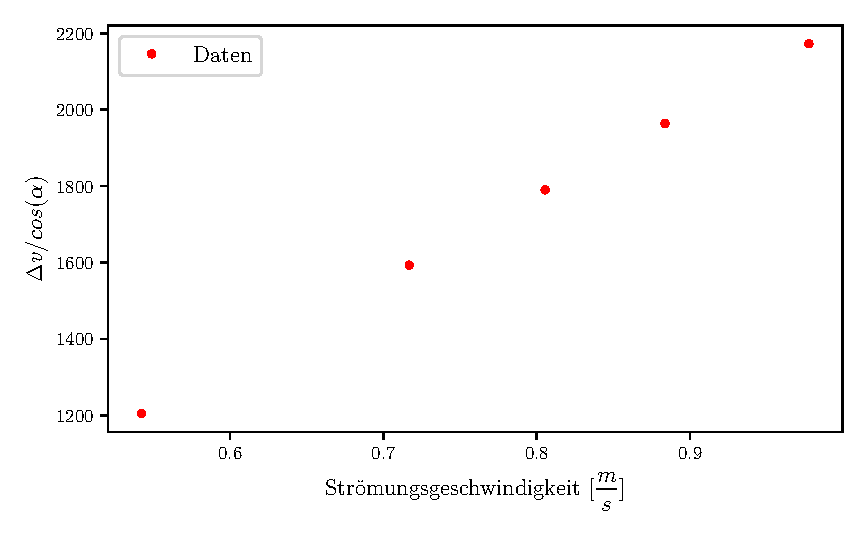
\includegraphics[width=0.7\textwidth]{build/plot1.pdf}
  \caption {Messwerte der Justagemessung zur Bestimmung der Halbwertsbreite und der optimalen Verzögerung zwischen den beiden PMTs.}
  \label{fig:Verzoegerung}
\end{figure}
Der Graph zur Justierung der Verzörgerungsleitungen in \autoref{fig:Verzoegerung} weist ein leichtes Plateau auf.
Dieses Plateau ist, wie in der Durchführung beschrieben, auf die normierte Pulsdauer der Ausgangssignale der Diskriminatoren zurückzuführen und befindet sich im erwarteten Bereich von \SI{10}{\nano \second}. \\
Zur Bestimmung der Halbwertsbreite wird zunächst die Höhe des Plateaus
\begin{align*}
    I_{Plateau} = (21.40 \pm 0.6) \si{\second^{-1}}
\end{align*}
berechnet, indem das arithmetische Mittel und Standardabweichung von dem Werten des Plateaus bestimmt wird.
Außerdem werden an beiden Seiten ein lineraer Fit eingefügt.
Die berchneten Parameter ergeben sich zu 
\begin{align}
  a_l &= (2.28 \pm 0.08)  \si{\nano\second^{-1}\second^{-1}} & b_l &= (42.06 \pm 1.11) \si{\second^{-1}} \\
  a_r &= (-2.15 \pm 0.04) \si{\nano\second^{-1}\second^{-1}} & b_r &= (56.03 \pm 0.73) \si{\second^{-1}}.
\end{align}
Danach wird die Halbwertsbreite bestimmt, indem die Schnittpunkte der Hälfte der mittleren Höhe des Plateaus mit den beiden Fits an der Seite zu
\begin{align*}
   \Delta t = t_r - t_l = (34.8 \pm 0.8) \si{\nano\second}
\end{align*}
berechnet werden.
Hää was genau hast du hier gemacht? Dachte du hättest hier den Schnitpunkt der Fits berechnet... warum abgelesen?
Durch die abgelesenen Schnittpunkte mit den beiden Flanken lässt sich nun die Verzögerungszeit zu
\begin{equation}
  \symup{\Delta}t_K = 40 - \left[ |-25 \pm 0.5| + |18 \pm 0.5| \right] \si{\nano\second} = \- 3 \pm 0.71\; \si{\nano\second}
\end{equation}
bestimmen. Dabei ergeben sich die \SI{40}{\nano\second} aus der Summation der Breiten der beiden Diskriminatoren.

\subsection{Kalibration}
\label{subsec:Kalibration}
Um den Vielkanalanalysator zu kalibrieren werden mit Hilfe eines Doppelimpuls-Generators Impulse
mit unterschiedlichem zeitlichem Abstand eingelesen. Die belegten Kanäle sind in \autoref{fig:plot2} dargestellt und gegen die Impulsabstände aufgetragen.
\begin{figure}[H]
  \centering
  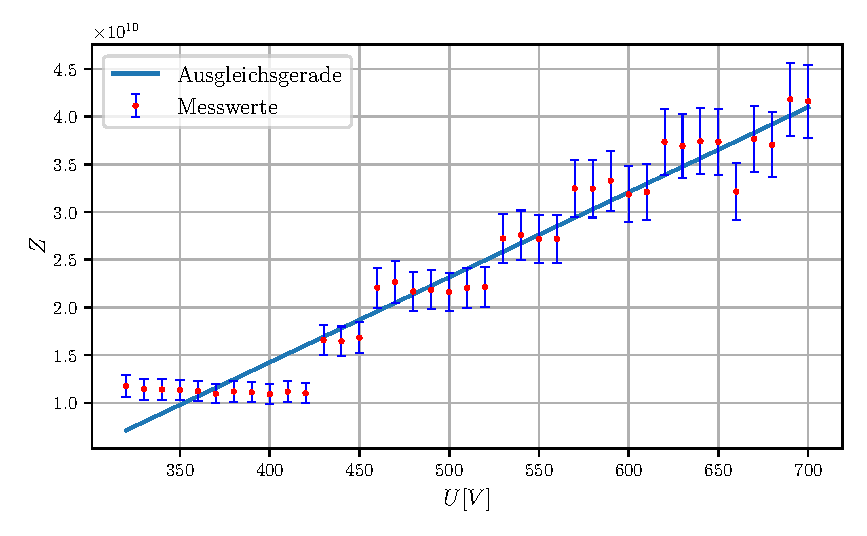
\includegraphics[width=0.7\textwidth]{build/plot2.pdf}
  \caption {Messwerte und Ausgleichsgerade der Kalibrationsmessung zur Umrechnung von Kanalnummern in Zerfallszeiten.}
  \label{fig:plot2}
\end{figure}
Außerdem wurde ein linearer Fit angelegt und die Parameter zu
\begin{align}
  a_k &= (46.00 \pm 7.75) \si{\nano\second^{-1}\second^{-1}} & b_k &= (-6.00 \pm 4.36) \si{\second^{-1}}
\end{align}
berechnet.

\subsection{Berechnung des Unntergrunds}
\label{subsec:Untergrund}

Bei der Messmethode, die in \autoref{subsec:Messmethode} beschrieben wurde, kann es zu Messfehlern kommen, wenn in der eingestellten Suchzeit
\begin{align}
  T_S = 10 \si{\micro\second}
  \label{eqn:Suchzeit}
\end{align}
ein weiteres Myon in den Tank eintrifft, was dann zu einem falschen Stoppsignal führt. 
Es tritt somit ein Untergrund über die gesamte Messzeit
\begin{align}
  T_{ges} = 169,832.86 \si{\second},
  \label{eqn:Messzeit}
\end{align}
auf, der sich gleichmäßig auf die Kanäle aufteilt, aufgrund der Unabhängigkeit der Myonen.
Die Wahrscheinlichkeit, dass $n$ Myonen bei einem Erwartungswert
\begin{align*}
  \mu(T_S) = I_{Mess} T_S
  \label{eqn:Erwartungswert}
\end{align*}
in der Zeit $T_S$ in den Detektor einfallen ist poissonverteilt
\begin{equation}
  p_{\mu} = \frac{\mu}{n!} \text{e}^{-\mu}.\label{eqn:Poission}
\end{equation}
Die durchschnittlich gemessene Rate $I_{Mess}$ lässt sich mit
\begin{align*}
  I_{Mess} = \frac{N_{Start}}{T_{ges}} = (27.95 \pm 0.01) \si{\second}^{-1}
\end{align*}
berechnen, wobei $N_{Start}$ die gesamt Anzahl der Startimpulse 
\begin{align*}
  N_{Start} = (4747339 \pm 2178.84) 
\end{align*}
ist.
Der gesamte Untergrund ergibt sich nun aus \autoref{eqn:Poission} für ein Teilchen und der Anzahl der Startimpulse zu
\begin{align}
  U_{ges} = p_{\mu}(1) N_{Start} = (1326.70 \pm 1.20).
\end{align}
Dieser Untergrund muss nun auf die relevanten Kanäle normiert werden. Dabei beträgt die Anzahl der relevanten Kanäle in $T_S$ $435$ und somit ergibt sich der Untergrund zu
\begin{align}
  U_n = \frac{U_{ges}}{435} = (3.050 \pm 0.003).
\end{align}

\subsection{Lebenszeit der Myonen}
\label{subsec:Lebenszeit}
Die Counts pro zeitintervall wird in \autoref{fig:plot3} dargestellt.
\begin{figure}[H]
  \centering
  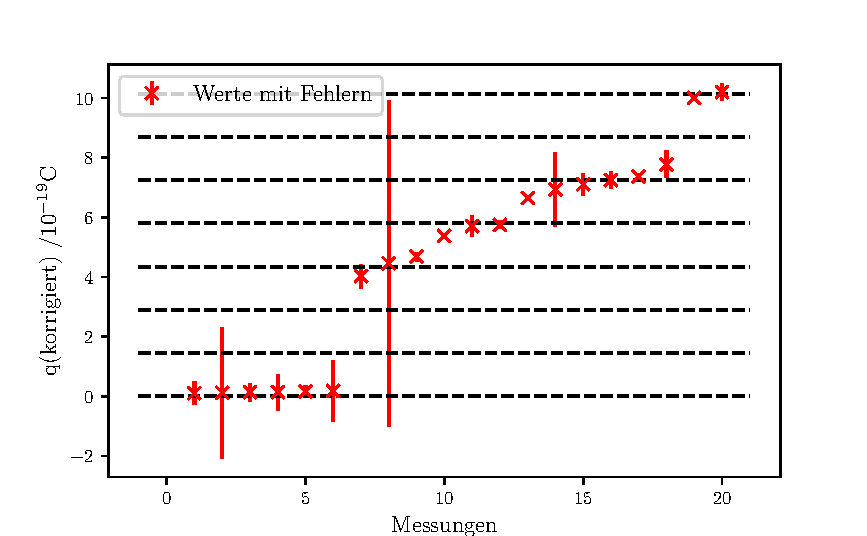
\includegraphics[width=0.7\textwidth]{build/plot3.pdf}
  \caption {Messwerte und Exponentialfit, welcher den Untergrund Un als Fitparameter berücksichtigt, der Lebensdauer-Messung..}
  \label{fig:plot3}
\end{figure}